% Fig. 2 : Optimal angle determination (case of 4-QAM) -- dessinee en TikZ
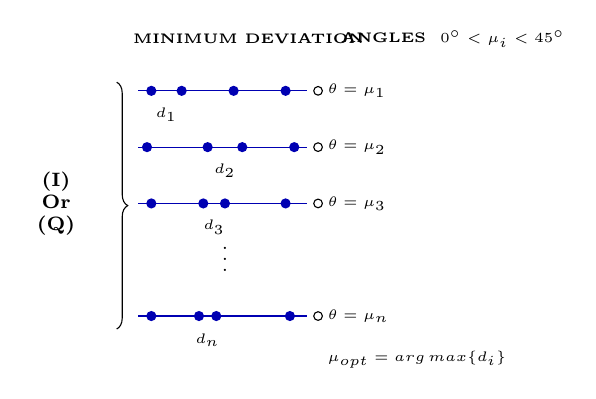
\begin{tikzpicture}[x=0.55cm,y=0.55cm,font=\scriptsize,
  dot/.style={circle,fill=blue!70!black,inner sep=1.3pt},
  lab/.style={font=\tiny\bfseries,inner sep=1pt}]
  % en-tetes
  \node[lab,anchor=west] at (-0.2,6.4) {MINIMUM DEVIATION};
  \node[lab,anchor=west] at (4.6,6.4) {ANGLES\ \ $0^\circ<\mu_i<45^\circ$};
  % accolade (I) or (Q)
  \draw[decorate,decoration={brace,amplitude=4pt,mirror}] (-0.5,-0.3) -- (-0.5,5.4);
  \node[font=\scriptsize\bfseries,align=center] at (-1.9,2.6) {(I)\\Or\\(Q)};
  % lignes : (y, x1,x2,x3,x4, indice, position de d_i)
  \foreach \y/\a/\b/\c/\d/\i/\m in {5.2/0.3/1.0/2.2/3.4/1/0.65, 3.9/0.2/1.6/2.4/3.6/2/2.0,
                                    2.6/0.3/1.5/2.0/3.4/3/1.75, 0.0/0.3/1.4/1.8/3.5/n/1.6}{
    \draw[blue!70!black] (0,\y) -- (3.9,\y);
    \foreach \x in {\a,\b,\c,\d} \node[dot] at (\x,\y) {};
    \node[lab] at (\m,\y-0.55) {$d_\i$};
    \node[lab,anchor=west] at (4.3,\y) {$\theta=\mu_\i$};
    \draw (4.15,\y) circle (0.1);
  }
  \node at (2,1.5) {$\vdots$};
  \node[lab,anchor=west,align=left] at (4.1,3.2) {};
  \node[lab,anchor=west] at (4.3,-1.0) {$\mu_{opt}=\operatorname{arg\,max}\{d_i\}$};
\end{tikzpicture}
